\section{Active learning calibration}
\label{app:al}

This calibration was run on WikiANN-sq before the annotated corpus existed, to establish
whether the acquisition strategy comparison could resolve a difference at all. It is
reported here rather than in the body because it measures the experimental design rather
than the corpus: the answer turned out to be that at three seeds the design cannot resolve
differences below roughly 0.04, which is a fact about the method and not a finding about
Albanian.

Table~\ref{tab:al} reports a calibration sweep on WikiANN-sq: two acquisition strategies,
three seeds, five annotation budgets, 30 model trainings in total.

\begin{table}[htbp]
\centering
\caption{Active learning on WikiANN-sq. Mean $F_1 \pm$ standard deviation over three seeds.}
\label{tab:al}
\begin{tabular}{lcc}
\toprule
Labelled sentences & Random & Uncertainty \\
\midrule
250  & 0.685 $\pm$ 0.000 & 0.692 $\pm$ 0.016 \\
500  & 0.863 $\pm$ 0.017 & 0.847 $\pm$ 0.017 \\
750  & 0.882 $\pm$ 0.007 & 0.858 $\pm$ 0.019 \\
1000 & 0.883 $\pm$ 0.029 & 0.888 $\pm$ 0.025 \\
1250 & 0.898 $\pm$ 0.004 & 0.906 $\pm$ 0.012 \\
\bottomrule
\end{tabular}
\end{table}

\begin{figure}[htbp]
\centering
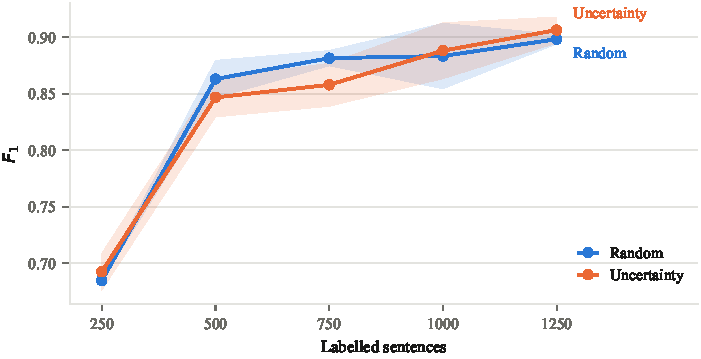
\includegraphics[width=\linewidth]{images/fig_learning_curve}
\caption{Active learning on WikiANN-sq. Shaded bands are $\pm$ one standard deviation
across three seeds; they overlap at every budget.}
\label{fig:al}
\end{figure}

No budget shows a significant difference. The largest gap, 0.024 at 750 sentences, reaches
$t = -2.03$ against the $|t| > 2.8$ required at three seeds. The direction of the
difference also alternates --- uncertainty leads at three of five budgets and random at two
--- which is characteristic of noise rather than of an effect.

Uncertainty sampling is slightly \emph{worse} at intermediate budgets. This is consistent
with a known property of entropy-based acquisition: it favours atypical and difficult
sentences, which early in training are unrepresentative of the test distribution.

The practical consequence is a detection threshold. With three seeds at these budgets, a
strategy difference below approximately 0.04 cannot be distinguished from seed variance.
Any conclusive claim would require more seeds or wider budget spacing.



\section{Corpus construction detail}
\label{app:corpus}

\begin{table}[htbp]
\centering
\caption{Sentences discarded during corpus construction (2\,687 candidates).}
\label{tab:filter}
\begin{tabular}{lr}
\toprule
Reason & Count \\
\midrule
Fragment with unbalanced brackets & 71 \\
Fourth or later member of a stub template family & 22 \\
Split word (e.g.\ \emph{Andre}~+~\emph{w}) & 18 \\
Exact duplicate & 5 \\
Split hyphenated name (\emph{Dommartin-au}~+~\emph{x-Bois}) & 2 \\
\midrule
Total & 120 (4.5\%) \\
\bottomrule
\end{tabular}
\end{table}

\begin{table}[htbp]
\centering
\caption{Corpus comparison. Both derive from Albanian Wikipedia.}
\label{tab:corpora}
\begin{tabular}{lrrl}
\toprule
Corpus & Sentences & Median tokens & Construction \\
\midrule
WikiANN-sq (train) & 5\,000 & 6 & automatic link projection \\
This work & 2\,500 & 20 & sampled, filtered, hand-verified \\
\bottomrule
\end{tabular}
\end{table}

\begin{figure}[htbp]
\centering
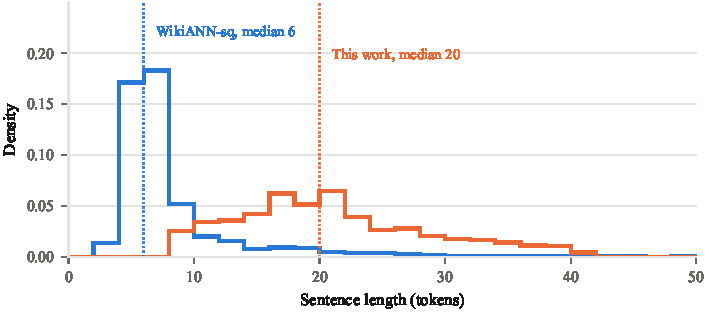
\includegraphics[width=\linewidth]{images/fig_corpus_lengths}
\caption{Sentence-length distributions. WikiANN-sq is dominated by short fragments;
the corpus built here has a median of 20 tokens.}
\label{fig:corpus}
\end{figure}

\section{Error composition}
\label{app:errors}

\begin{figure}[htbp]
\centering
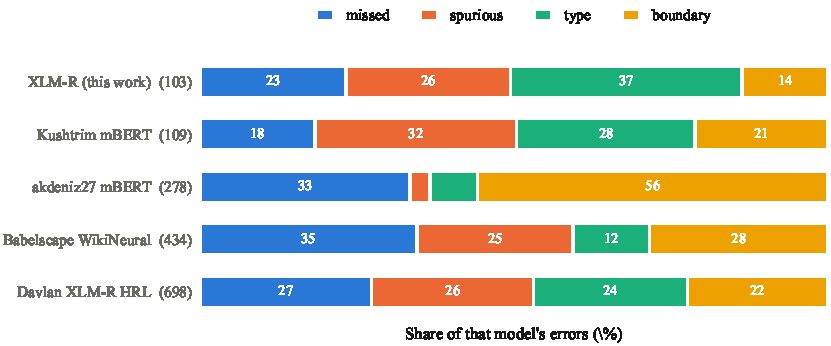
\includegraphics[width=\linewidth]{images/fig_errors}
\caption{Error composition per model; the total error count is in parentheses.
Categories are mutually exclusive and sum to 100\%.}
\label{fig:errors}
\end{figure}

\section{Per-seed fine-tuning detail}
\label{app:finetune}

\begin{table}[htbp]
\centering
\caption{Fine-tuned on the gold training split. The bracketed interval is a bootstrap CI
over test sentences for the best-dev seed; $\pm$ is run-to-run variance across seeds.}
\label{tab:gold-finetune}
\begin{tabular}{lccc}
\toprule
Seed & dev $F_1$ & test $F_1$ & \\
\midrule
1 & 0.774 & 0.723 & [0.660, 0.782] \\
2 & 0.747 & 0.728 & \\
3 & 0.770 & 0.677 & \\
\midrule
Mean & & \multicolumn{2}{l}{0.709 $\pm$ 0.028} \\
\bottomrule
\end{tabular}
\end{table}
